% INSTRUCTION FOR LLM:
% 1. Keep the multiline writing style and keep minimal diff when editing. If possible dont rewrite all text but
% edit only the relvent line. Avoid merging lines into one.
\documentclass[final,5p,times,twocolumn]{elsarticle}


\usepackage{amssymb}
\usepackage{amsmath}
\usepackage{url}
\usepackage[colorlinks=true, urlcolor=blue, linkcolor=blue, citecolor=blue]{hyperref}

\DeclareRobustCommand{\secref}[1]{\hyperref[#1]{Section~\ref*{#1}}}
\DeclareRobustCommand{\figref}[1]{\hyperref[#1]{Figure~\ref*{#1}}}
\DeclareRobustCommand{\figsref}[2]{\hyperref[#1]{Figures~\ref*{#1}} and~\hyperref[#2]{\ref*{#2}}}
\DeclareRobustCommand{\eqnref}[1]{\hyperref[#1]{Eq.~(\ref*{#1})}}

\renewcommand{\ttdefault}{lmtt}

\journal{High Energy Density Physics}

\begin{document}

\begin{frontmatter}

%% Title, authors and addresses

\author{Roee Yaron$^{1,2}$}
\author{Ehud Nakar\corref{cor1}$^2$}
\ead{nakar@tauex.tau.ac.il}

\cortext[cor1]{Corresponding author}

\affiliation{organization={1. Israel Atomic Energy Commission},
           addressline={P.O. Box 7061}, 
           city={Tel Aviv},
           postcode={61070}, 
           state={},
           country={Israel}}
\affiliation{organization={2. School of Physics and Astronomy, Tel Aviv University},
           addressline={},
           city={Tel Aviv},
           postcode={6997801}, 
           state={},
           country={Israel}}

\title{Rosseland Mean Opacity for Expansion Opacity from Bound-Bound Lines} %% Article title

%% Abstract
\begin{abstract}
We define "Expansion Rosseland mean opacity" a new method for calculating Rosseland mean opacity that accounts for expansion
opacity, of bound-bound atomic transitions smoothed out due to the Doppler effect.
The method smooths the frequency-dependent opacity using a $\tau=1$ window, where for each frequency the
distance required to reach optical depth unity is calculated. The smoothed opacity is then determined from
$\kappa = 1/(\rho \Delta x)$, where $\Delta x$ is the path length for $\tau=1$. Monte Carlo radiative transfer simulations
using this new Rosseland opacity yield results similar to full frequency-group calculations, demonstrating that the averaging
successfully captures the essential physics of expansion opacity, while saving most of the MC computational cost.
\end{abstract}

%% Keywords
\begin{keyword}
%% keywords here, in the form: keyword \sep keyword

opacity \sep  Rosseland mean \sep expansion opacity \sep bound-bound transitions \sep kilonova \sep supernovae

\end{keyword}

\end{frontmatter}

%% main text

\section{Introduction}
\label{SecIntro}

    The interaction between radiation and matter is primarily determined by the material properties such as composition, density,
    and temperature, as well as the spectral characteristics of the radiation.
    In expanding plasmas, due to the Doppler effect, as photons travel through the plasma, their frequency changes. 
    This effect is mainly important for bound-bound transitions, due to their high gradient in frequency which cause photons to interact 
    with different lines as they travel through the plasma.
    This effect is known as expansion opacity, and it is important for many astrophysical applications, such as Type Ia supernovae,
    kilonovae and stellar winds. 
    Under the reasonable condition of non-ultra relativistic velocities, 
    the frequency shift due to the Doppler shift is approximately $\Delta \nu = \nu_0 \frac{\Delta v}{c}$.

    For non-moving plasmas, the radiation flux can be approximated well using the Rosseland mean opacity, which is a weighted
    average of the opacity over all frequencies. However, for expanding plasmas with significant bound-bound opacity, the Rosseland mean 
    opacity is not a good approximation, since the width of the bb lines is negligible and photons interact with them only due to their
    frequency change as they travel through the plasma. 
    Therefore the average distance a photon travels cannot be derived from $\kappa(\nu)$
    alone because it inherently depends on the photon's direction of movement and the plasma's velocity gradient.
    To avoid this problem and to allow calculation of transport that can inherently depend on the photon's direction of movement and
    velocity gradient, radiation transport in systems with expansion opacity is usually calculated using Monte Carlo simulations,
    which track individual photons and their frequency evolution as they propagate through the expanding medium.

    Calculating the Rosseland mean opacity has several motivations: a single opacity value (1) is required for analytic 
    models and closed-form solutions, which cannot treat full frequency-dependent opacity; (2) gives direct physical 
    intuition for how temperature and composition affect the opacity and hence the light curve; and (3) enables 
    faster and simpler simulations than full frequency-dependent calculations. 

    Previous attempts to address this problem have been proposed. Fontes et al. \cite{fontes2015opacity,fontes2017linesmeared}
    suggested using artificial 
    line broadening by assigning a line width corresponding to unphysical high temperature of 20 MeV, 
    which effectively smears the bound-bound lines 
    over a finite frequency range. This approach preserves the integral of the opacity over
    frequency (area-preserving line profiles) and for NSM ejecta it  
    produces frequency-dependent opacities that are one to two orders of magnitude greater than those
    obtained with expansion opacities in 
    the Sobolev approximation without broadening. Fontes et al. \cite{fontes2020opacity} demonstrated that
    their smeared opacity tables, 
    calculated using the Sobolev formalism, yield light curves for multigroup radiative transfer simulations
    that are similar to those 
    obtained from full line-by-line Monte Carlo radiation transport (using the superNu code) for kilonovae (neutron
    star mergers).
    However, this approach still requires multigroup frequency-dependent opacity tables rather than
    a single gray (frequency-averaged) Rosseland mean opacity and uses unphysical assumption which
    have been verified only for specific ejecta.
    Several works \cite{deprince2024kilonova,just2022properties,tanaka2020systematic} have shown how opacity depends on composition,
    temperature, density, and time by comparing the Planck mean expansion opacity over those parameters.
    The Planck mean is nevertheless a poor indicator of the "effective opacity" which sets the rate at which energy leaks out of the ejecta.
    In a non-expanding medium the frequency weighting that sets the typical photon escape is exactly the Rosseland mean, while in an expanding
    medium the relevant average should be at least of the same character and therefore not the Planck mean.

    In this paper we present a parameter "The expansion Rosseland mean opacity" that properly accounts for expansion opacity 
    effects from bound-bound lines. The method assumes a photon which travels "outwards" from the center of the expanding plasma and
    assumes homologous expansion ($r=v\cdot t $) and thus gives the opacity as a function of time in addition to the density and
    temperature $ \kappa (T, \rho, t) $.

    The structure of the paper is as follows: In \secref{SecExpansion} we describe how the expansion opacity is calculated, 
    and define the expansion Rosseland mean opacity.
    In \secref{SecRosseland}, we show the variation of the expansion Rosseland mean opacity with composition, temperature, density, and time
    and show how it scale differently from the Planck mean and discuss its physical meaning.
    In \secref{SecValidation} we demonstrate the use of the expansion Rosseland mean opacity in radiative transfer simulations and compare the
    results to the full frequency-group calculations. 
    In \secref{SecSummary} we summarize the results and discuss future work.
%which means that the time is the velocity and frequency gradient $t = \frac{dv}{dR} = \frac{d\nu}{dR}$.


\section{Expansion Opacity}
    \label{SecExpansion}
    
    The total opacity $\kappa$ is the sum of contributions from different physical processes:
    \begin{equation}
    \kappa = \kappa_{\mathrm{T}} + \kappa_{\mathrm{ff}} + \kappa_{\mathrm{bf}} + \kappa_{\mathrm{bb}}
    \end{equation}
    where $\kappa_{\mathrm{T}}$ is Thomson scattering, $\kappa_{\mathrm{ff}}$ is free-free opacity, $\kappa_{\mathrm{bf}}$ is 
    bound-free opacity (which we neglect in this work), and $\kappa_{\mathrm{bb}}$ is bound-bound opacity from atomic line 
    transitions.

    The bb opacity $\kappa_{\mathrm{bb}}$ depends on the plasma's ionization and excitation populations for each material. This is 
    calculated using the Boltzmann distribution.

    \begin{equation}
    N_{m,i+1} = \frac{N_{m,i}}{N_{m,0}} \frac{Z_{m,i+1}}{Z_{m,i}} \exp\left(-\frac{E_{i+1}-E_i}{kT}\right) \cdot g_{e}
    \end{equation}
    where $m, i, j$ are the indexes of the material, ionization level and energy level respectively, $N$ is the number density, $g$
    and $E$ are the degeneracy and energy of the energy level respectively, $k$ is the Boltzmann constant, $T$ is the temperature and 
    $g_e$ is the constant factor $g_e = \left(\frac{2\pi m_e kT}{h^2}\right)^{3/2}$.

    $Z_{m,i}$ is the partition function of the state $i$ for the material $m$, and is calculated using the partition function formula:
    \begin{equation}
    Z_{m,i} = \sum_{j} g_j \exp\left(-\frac{E_j}{kT}\right)
    \end{equation}

    The number density $N_{m, i}$ is calculated using the Saha equation.
    \begin{equation}
    \frac{N_{m, i}}{N_{m, 0}} = \frac{g_i}{g_0} \left(\frac{2\pi m_e kT}{h^2}\right)^{3/2} \exp\left(-\frac{E_i}{kT}\right)
    \end{equation}
    where $m_e$ is the electron mass.

    The optical depth of the bound-bound line is then calculated using the Sobolev approximation.
    \begin{equation}
        \tau_{j_l,j_u} = \frac{\pi e^{2}}{m_{e}} \frac{f_{j_l,j_u}}{\nu_{j_l,j_u}} t \left(N_{m,i,j_l} - \frac{g_{j_l}}{g_{j_u}} N_{m,i,j_u}\right)
    \end{equation}
    where $j_l$ and $j_u$ are the lower and upper energy levels respectively, $f_{j_l,j_u}$ is the oscillator strength of the transition 
    from the energy level $j_l$ to the energy level $j_u$, $\nu_{j_l,j_u}$ is the frequency of the transition, $N_{m,i,j_l}$ and $N_{m,i,j_u}$ 
    are the number densities of the lower and upper levels respectively, $g_{j_l}$ and $g_{j_u}$ are their degeneracies, and $t$ is the time from explosion.

    Then, there are two values for the bound-bound opacity, saturated and unsaturated which are calculated as:
    \begin{equation}
        \kappa_{bb,saturated}(\nu) = \sum_l \frac{\nu_l}{\rho c t} \delta(\nu - \nu_{l}) \cdot (1 - \exp(-\tau_{j_l,j_u}))
    \end{equation}
    \begin{equation}
        \kappa_{bb,unsaturated}(\nu) = \sum_l \frac{\nu_l}{\rho c t} \delta(\nu - \nu_{l}) \cdot \tau_{j_l,j_u}
    \end{equation}

    The saturated opacity gives the effective contribution of a narrow line in a larger frequency bin,
    by capping its effect once it becomes optically thick, since a singel line has a maximal effect on the opacity
    once all photons in the line's frequnecy are absorbed.
    The unsaturated opacity gives the real opacity at each point and for discrete frequency bins the 
    exact optical depth of a photon which travels through the entire frequency bin.
    The Expansion Rosseland opacity is calculated from the average distance an outward travelling
    photon goes through in a plasma before reaching optical depth of 1, i.e. being scattered or absorbed.
    This distance is calculated using the unsaturated opacity.

    An outward travelling photon with frequency $\nu_0$, will reach a new spectral line with frequency 
    $\nu_{l}$ after a velocity shift of $\Delta v = -c \ln(\nu_0/\nu_{l})$ which corresponds to a
    distance of $\Delta x = -c t \ln(\nu_0/\nu_{l})$.

    For that we define the cumulative frequency optical depth as:
    \begin{equation}
        \tau(\nu) = \int \kappa(\nu) \rho \, dx = ct \int \kappa(\nu) \rho \frac{d\nu}{\nu}
    \end{equation}
    And for each frequency $\nu_i$, given the frequency $\nu_j$ so that $\tau(\nu_j) - \tau(\nu_i) = 1$,
    we define the effective expansion opacity as:
    \begin{equation}
        \label{eq:kappa_eff_simple}
        \kappa_{eff}(\nu_i) = \frac{1}{\rho \Delta R} = \frac{1}{\rho ct \frac{\nu_j - \nu_i}{\nu_i}}
    \end{equation}

    For finite size frequency bins this process is done by interpolating between the frequency bins.
    This is needed since otherwise the frequency shift would have an artificial minimum of
    $\Delta \nu = \nu_{i+1} - \nu_i$, which would create an artificial opacity maximum of
    $\frac{1}{\rho ct \frac{\nu_{i+1}-\nu_{i}}{\nu_{i}}}$.
    
    Numerically, after discretizing the frequency, the stopping bin is found with the unsaturated
    optical depth by finding the first bin $j$ such that
    \begin{equation}
        \tau(\nu_{j-1}) - \tau(\nu_i) < 1,
        \qquad
        \tau(\nu_j) - \tau(\nu_i) > 1
    \end{equation}
    This choice is made with the unsaturated opacity because it identifies where the photon would
    actually reach optical depth unity. The sub-bin position is then estimated with the saturated
    opacity of bin $j$, which gives the effective contribution of the lines inside the finite bin.
    If this saturated contribution is large enough to reach unity inside the bin, we use
    \begin{equation}
        \Delta \nu_{\tau=1} = \nu_{j-1} - \nu_i + (\nu_j - \nu_{j-1})
        \frac{1 - (\tau(\nu_{j-1})-\tau(\nu_i))}{\Delta\tau^{s}_j},
    \end{equation}
    where $\Delta\tau^{s}_j$ is the optical depth of bin $j$ calculated from the saturated opacity.
    If it is not large enough, we set $\Delta\nu_{\tau=1}=\nu_j-\nu_i$. When one bin alone determines
    the opacity, we use the saturated opacity of that bin:
    \begin{equation}
        \label{eq:kappa_eff}
        \kappa_{eff}(\nu_i) = \frac{ \sum_l (1 - \exp(-\tau(\nu_l)))}{\rho ct \frac{\nu_{i+1}-\nu_{i}}{\nu_{i}}} + \kappa_{\mathrm{T}} + \kappa_{ff}(\nu_i)
    \end{equation}
    This interpolation is approximate, but it avoids summing over all individual lines, which are
    often orders of magnitude more numerous than the frequency bins. The result is accurate when
    $\Delta\tau \ll 1$ or $\Delta\tau \gg 1$. For the intermediate case, $\Delta\tau \sim 1$, it
    introduces a small error which should mostly cancel on average.

    \figref{fig:BB_line_example} shows the unsaturated opacity, saturated opacity, and effective
    expansion opacity of iron after 3 days, for density $1 \times 10^{-12}$~g/cm$^3$ and temperature
    0.5~eV.
    %Top: frequency-dependent opacity showing unsaturated opacity, saturated opacity, and effective
    %expansion opacity. Bottom: zoom into a narrow photon-energy range with the same quantities.
    For species with $A<28$ in Type~Ia supernova compositions we use the atomic line data of Kurucz \& Bell
    (1995; CD~23) \cite{kurucz1995}. For kilonova composition, where the relevant nuclei have $A>28$, 
    we use the NIST Atomic Spectra Database \cite{nistASD}.

    % NOTE (editors / future AI): For vertically stacked panels use top/middle/bottom (not left/right). For a true side-by-side layout, left/right is fine. Do not set panel labels in \textbf{...}; keep them in normal weight.
    \begin{figure}[h]
        % How to create:
        % Script: plots/plot_kappa_smoothed_vs_raw.py
        % cd ~/Documents/PHD/URILIGHT/python_opac_calc2
        % python plots/plot_kappa_smoothed_vs_raw.py --png
        % mv kappa_smoothed_vs_raw.png build_paper/figs/kappa_smoothed_vs_raw.png
        % mv kappa_smoothed_vs_raw_error.png build_paper/figs/kappa_smoothed_vs_raw_error.png
        % (Two rows in the PDF: row~1 = first PNG; row~2 = zoomed opacity comparison.)
        \centering
        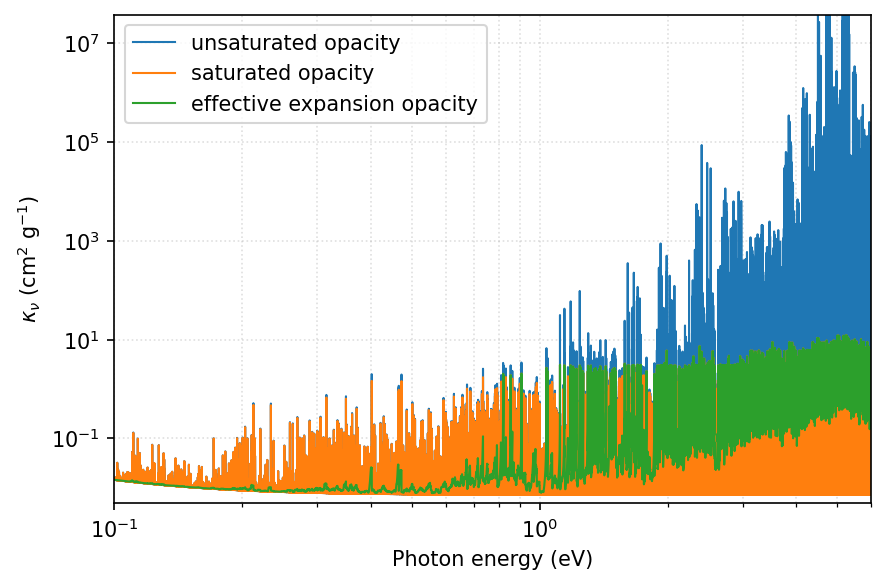
\includegraphics[width=\columnwidth]{figs/kappa_smoothed_vs_raw.png}\\[0.5em]
        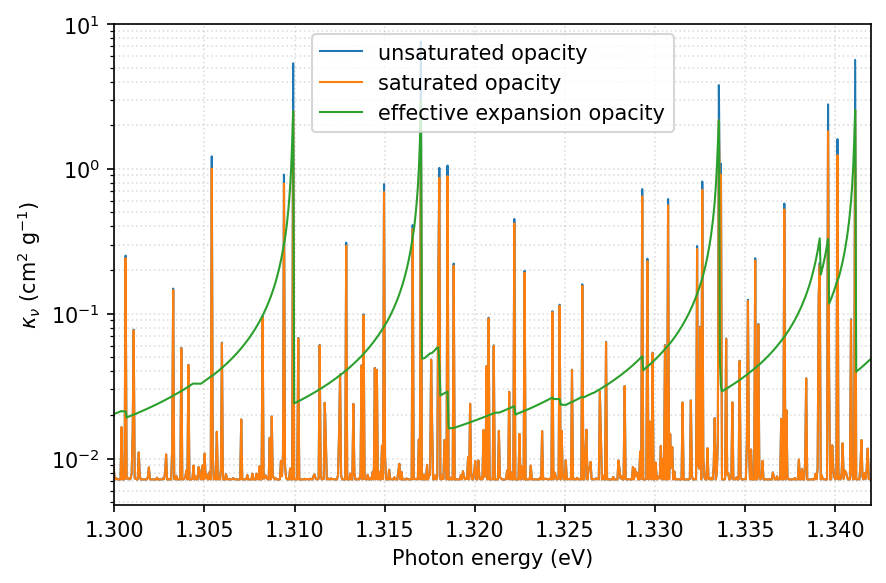
\includegraphics[width=\columnwidth]{figs/kappa_smoothed_vs_raw_error.png}
        \caption{Unsaturated opacity, saturated opacity, and effective expansion opacity, 
        for iron at $\rho = 1 \times 10^{-12}$~g/cm$^3$, $T = 0.5$~eV, $t = 3$~days.
        For large (top) and zoomed (bottom) energy ranges.}
        \label{fig:BB_line_example}
    \end{figure}

\section{Rosseland Mean of Effective Expansion Opacity}
    \label{SecRosseland}

    The Planck mean opacity is an emission-weighted average, while the Rosseland mean opacity is a 
    transport-weighted harmonic mean:
    \begin{equation}
        \kappa_P = \frac{\int \kappa_\nu B_\nu(T) d\nu}{\int B_\nu(T) d\nu},
        \qquad
        \frac{1}{\kappa_R} =
        \frac{\int \frac{1}{\kappa_\nu} \frac{\partial B_\nu(T)}{\partial T} d\nu}
        {\int \frac{\partial B_\nu(T)}{\partial T} d\nu}.
    \end{equation}
    where $B_\nu(T)$ is the Planck function.
    In this section these averages are applied to the frequency-dependent opacities defined above,
    including the effective expansion opacity.

    The main problem using the Rosseland opacity on the normal expansion opacity is that its BB contribution
    converge to zero for infninte bin resultion.
    \figref{fig:convergence} shows the convergence of the Rosseland mean opacity as a function of the
    frequency resolution $\Delta\nu/\nu$ (equivalent to the number of frequency bins in logarithmic resolution)
    for iron (Fe, Z=26) in top and erbium (Er, $Z = 68$) in bottom.
    Iron is an iron-group element with an open d-shell, representative of the heavy material in
    Type~Ia supernova ejecta. Erbium is a lanthanide with an open f-shell, which is common in
    kilonova compositions and gives a much larger bound-bound opacity than iron.
    In \figref{fig:convergence} we plot the Rosseland mean of the old saturated expansion opacity 
    (bin-by-bin use of \eqnref{eq:kappa_eff} with $(1 - \exp(-\tau(\nu_j)))$), 
    the Rosseland mean of the effective expansion opacity (\eqnref{eq:kappa_eff}), and the Planck mean opacity.
    The Planck mean is computed with the saturated expansion opacity on a 300-bin frequency grid and is nearly 
    independent of the number of bins. 
    Free-free and Thomson opacity are included so that the Planck and Rosseland means are comparable. 

    \begin{figure}[h]
    % How to create:
    % cd ~/Documents/PHD/URILIGHT/python_opac_calc2
    % python convergence_tests/plot_opac_vs_bins.py
    % mv convergence_Fe_rho1.00e-12_t3.0days.png build_paper/figs/
    %for Er, go to cluster
    % cd /mnt/lbosm1/home/roeey/SN/expansion_opacity_calculation
    % python plot_opac_vs_bins.py --composition Er --T 1.0 1e-12 1.0 --png
    % (Er panel: produce convergence_Er_rho1.00e-12_t1.0days.png and copy to figs/)
    % scp roeey@10.10.10.4:/home/roeey/LIGHTBITS/SN//expansion_opacity_calculation/convergence_Er_rho1.00e-12_t1.0days.png figs/
    \centering
    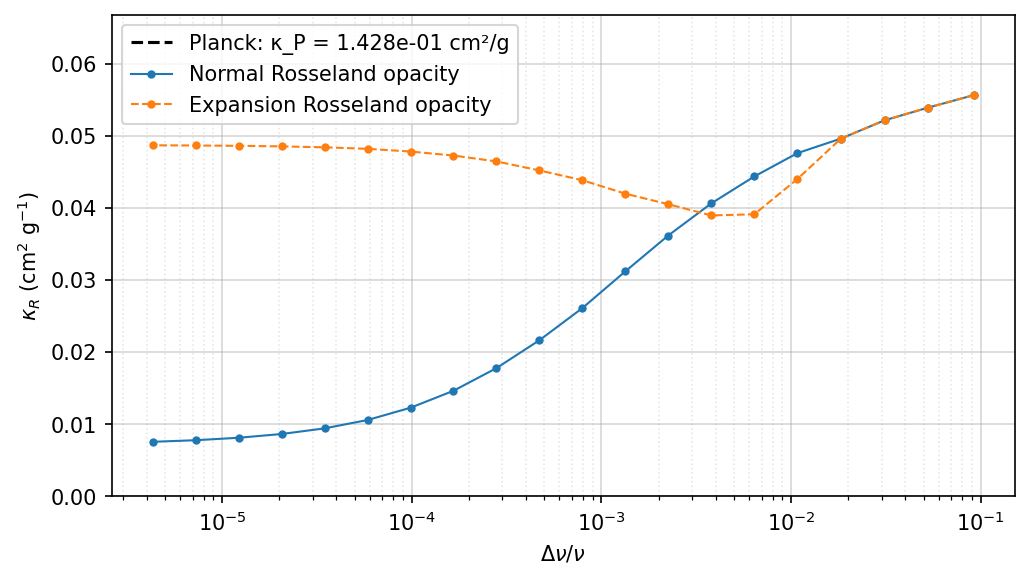
\includegraphics[width=\columnwidth]{figs/convergence_Fe_rho1.00e-12_t3.0days.png}\\[0.5em]
    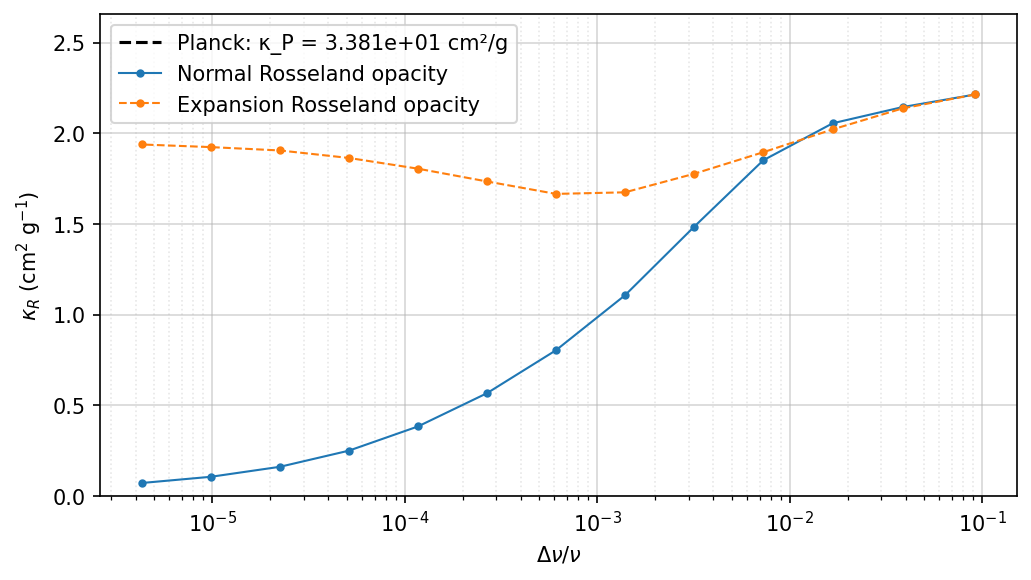
\includegraphics[width=\columnwidth]{figs/convergence_Er_rho1.00e-12_t1.0days.png}
    \caption{Convergence of the Rosseland mean opacity vs. the frequency resolution in $\Delta\nu/\nu$. 
    Top: iron for $\rho = 1 \times 10^{-12}$~g/cm$^3$, $T = 0.5$~eV, $t = 3$~days. 
    Bottom: erbium (lanthanide, $Z = 68$); $\rho = 1 \times 10^{-12}$~g/cm$^3$, $T = 1$~eV, $t = 1$~day. 
    In each panel: Rosseland mean of the saturated expansion opacity, Rosseland mean of the effective expansion opacity
    and Planck mean opacity written in the legend.}
    \label{fig:convergence}
    \end{figure}

    The results show that the expansion rosseland opacity is barely dependent on the frequency resolution
    and gives converged Rosseland opacity even for low resolutions (large bins) such as 
    $\Delta\nu/\nu \gtrsim 4\cdot 10^{-2}$ (which is equivalent to less than 200 bins for the full spectrum used).
    The reason the effective opacity gives correct results even for large bins is that the spectral lines are
    randomly distributed within each frequency bin. As long as the lines are randomly 
    distributed, \eqnref{eq:kappa_eff} provides a good approximation since it represents the typical distance
    a photon travels in a frequency bin. The fact that we observe good agreement between low-resolution and
    high-resolution calculations for the effective expansion Rosseland mean opacity for both iron and erbium confirms 
    that the line locations are indeed close enough to randomly distributed within the bins. 
    This also offers a rationale for the accuracy of the results done with the artificial line-broadening
    prescription of Fontes et al.\ \cite{fontes2015opacity,fontes2017linesmeared}: 
    spreading line opacity over frequency is analogous to many narrow lines at random positions within
    a coarse bin, so either picture can yield similar cumulative opacity in the bin, 
    consistent with smeared Sobolev tables reproducing Monte Carlo transport \cite{fontes2020opacity}.
    At low frequency resolution the Rosseland mean of the saturated expansion opacity is very close
    to the Rosseland mean of the effective expansion opacity. This happens because, when one bin alone
    determines the opacity, the effective expansion opacity is equivalent the saturated opacity of
    that bin.

    Using the formalism formerly described, we calculated the opacity of materials for different times, 
    densities and temperatures and constructed opacity tables that can be used for simulations of type~Ia
    supernova and kilonova.
    To mimic Type Ia ejecta, we used $^{56}$Ni and followed its decay chain,
    $^{56}{\rm Ni}\rightarrow{}^{56}{\rm Co}\rightarrow{}^{56}{\rm Fe}$, using the composition appropriate
    for each time window. We assumed the half-lives of 
    $t_{1/2}(^{56}{\rm Ni}) = 6.075$ days and $t_{1/2}(^{56}{\rm Co}) = 77.233$ days.
    For the kilonova case we used a reduced mixture,
    $X_{34}=0.5$, $X_{44}=0.15$, $X_{52}=0.25$, and $X_{68}=0.1$.
    Kilonova ejecta contain many elements, so this mixture was chosen to represent the main
    $p$-, $d$-, and $f$-block contributions without calculating every species.
    The block fractions were estimated from the $Y_e=0.2$ abundance distribution in
    Fig.~11 of Tanaka et al.\ \cite{tanaka2020systematic}; Se ($Z=34$) and Te ($Z=52$)
    represent the $p$-block, Ru ($Z=44$) the $d$-block, and Er ($Z=68$) the $f$-block.
    Within each block we selected elements with relatively large abundance.

    Since the Rosseland mean opacity is problematic to define for expansion opacity, previous works often
    used the Planck mean opacity to compare the opacity of different compositions in different temperatures.
    We check how well the Planck and the effective expansion Rosseland means are correlated by comparing
    their trends and their
    ratio as functions of temperature and density. \figsref{fig:rosseland_planck_ni}{fig:rosseland_planck_kilonova}
    show the Rosseland mean, Planck mean, and their ratio for
    nickel 56 decay chain and kilonova composition.
    In both compositions the Rosseland and Planck means usually decrease with density but their
    ratio vary between 1 to 30 and depends on the density and temperature. This means that the Planck mean opacity
    is not strongly correlated with the effective expansion Rosseland mean opacity.

    \iffalse
    To get an estimation on the time dependecy,
    we show in \figsref{fig:opac_rho_T}{fig:opac_rhot_T} for $^{56}$Ni the effective expansion Rosseland mean opacity 
    at three different times (1, 10, and 100 days) as a function of temperature and density (\figref{fig:opac_rho_T})
    and as a function of temperature and the product $\rho \cdot t$ (\figref{fig:opac_rhot_T}).
    It is apperent that the opacity decreases with time in a similar way to its decay with density,
    as expected for bound-bound transitions in expanding media. The $\rho \cdot t$ representation is more 
    natural for expanding media and better illustrates how the opacity scales with the expansion parameter.
    

    The opacity behavior shown in \figsref{fig:opac_rho_T}{fig:opac_rhot_T} can be understood
    from the expansion opacity formalism. From \eqnref{eq:kappa_eff_simple}, the effective opacity is
    $\kappa = 1/(ct \rho \Delta\nu/\nu)$. 
    For bound-bound dominated frequencies, photon absorption is mainly limited by saturated lines, 
    which will absorb the photon regardless of the 
    density or time since $\tau \gg 1$. In this regime, $\Delta\nu/\nu$ is approximately constant, and therefore 

    $\kappa \sim 1/(\rho \cdot t)$.

    However, the opacity shown in the figures deviates significantly from this simple scaling for several reasons. Firstly, the 
    bound-bound contribution is only important for certain frequency ranges, while at other frequencies free-free and Thomson 
    scattering dominate the opacity. Secondly, the Saha equation solution depends on density, and therefore the ionization fraction 
    changes with density, affecting the bound-bound line strengths. Thirdly, the time evolution changes the composition 
    ($^{56}$Ni to $^{56}$Co to $^{56}$Fe), which has slightly different opacities. These effects combine to produce 
    the complex behavior observed in the opacity maps.
    Still, the $\rho \cdot t$ representation in \figref{fig:opac_rhot_T} shows less time sensitivity than \figref{fig:opac_rho_T} 
    because the time dependence is largely absorbed into the scaling parameter, making the opacity behavior more uniform across 
    different times.

    We note that the Planck mean opacity used in expansion-opacity work is usually evaluated with the same saturation factor
    $1 - \exp(-\tau)$ as in Monte Carlo line interaction, because bound-bound absorption contributes to the total opacity in that
    saturated form rather than as the raw line opacity alone.

        \begin{figure}[h]
    \centering
    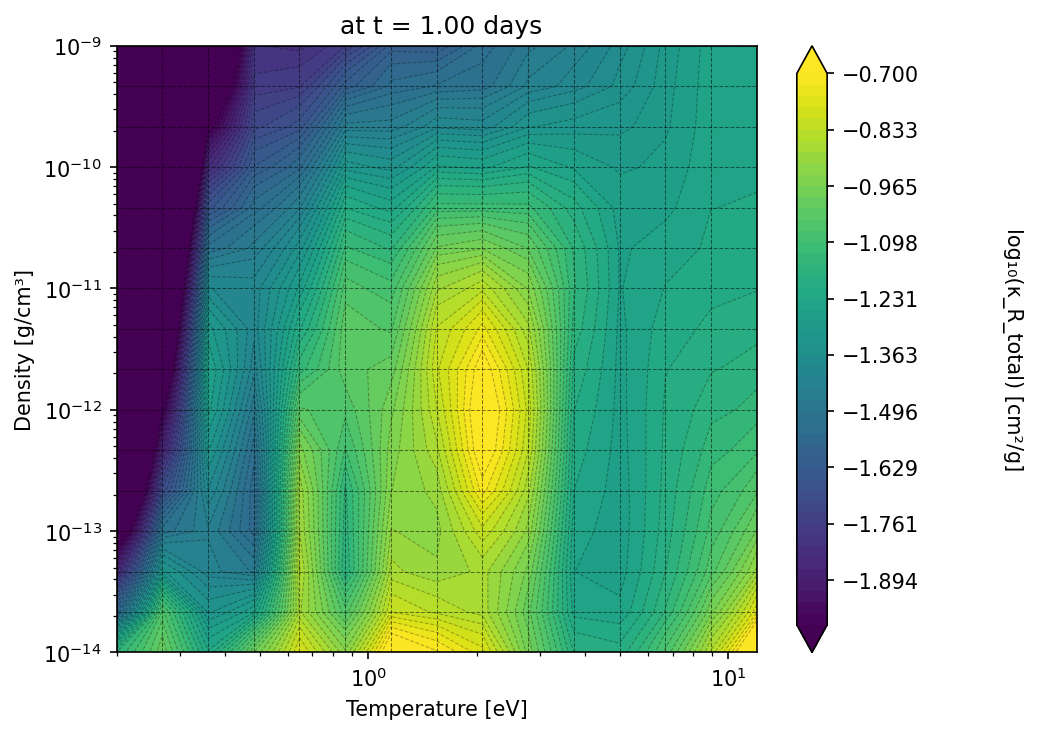
\includegraphics[width=\columnwidth]{figs/opac_map_rho_T/t_1days.png}\\[0.35em]
    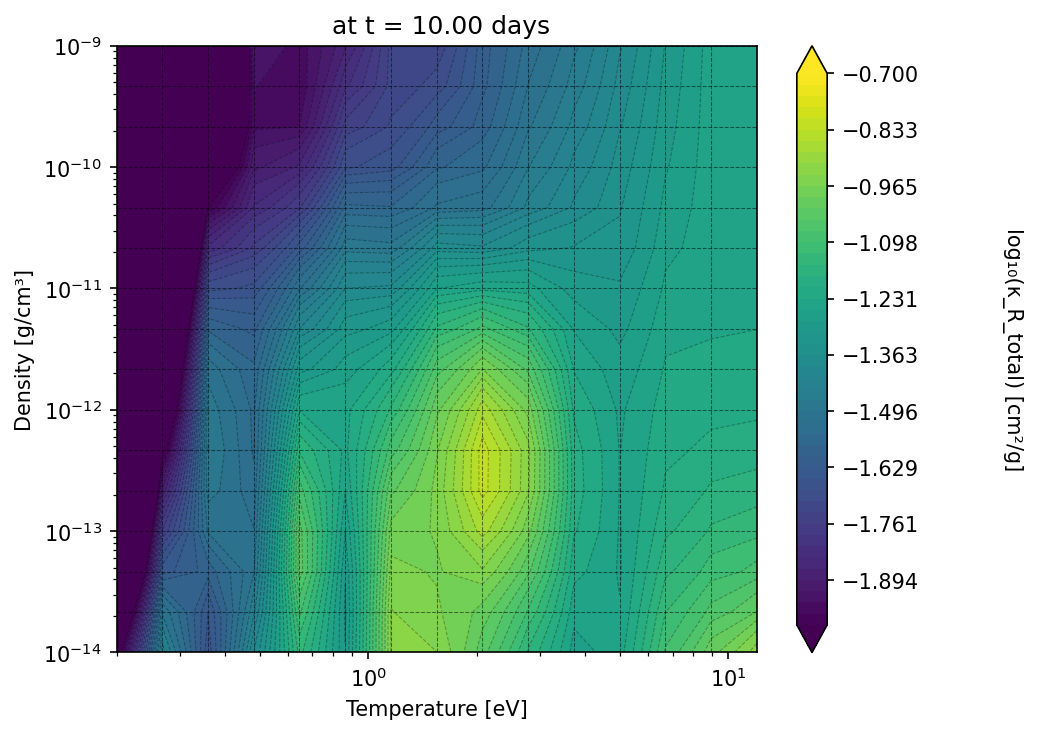
\includegraphics[width=\columnwidth]{figs/opac_map_rho_T/t_10days.png}\\[0.35em]
    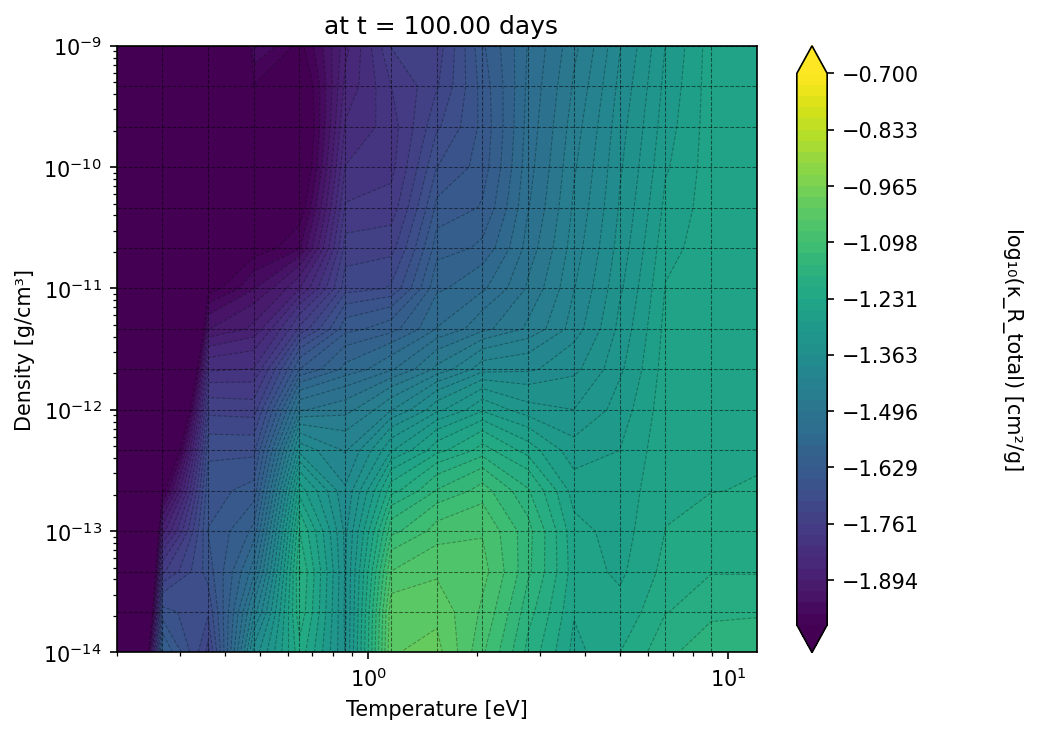
\includegraphics[width=\columnwidth]{figs/opac_map_rho_T/t_100days.png}
    \caption{Effective expansion Rosseland mean opacity for nickel as a function of temperature and density at t = 1, 10, and 100 days 
    (from top to bottom). The opacity is calculated using the expansion opacity formalism described in \secref{SecExpansion}.}
    \label{fig:opac_rho_T}
    \end{figure}



    \begin{figure}[h]
    \centering
    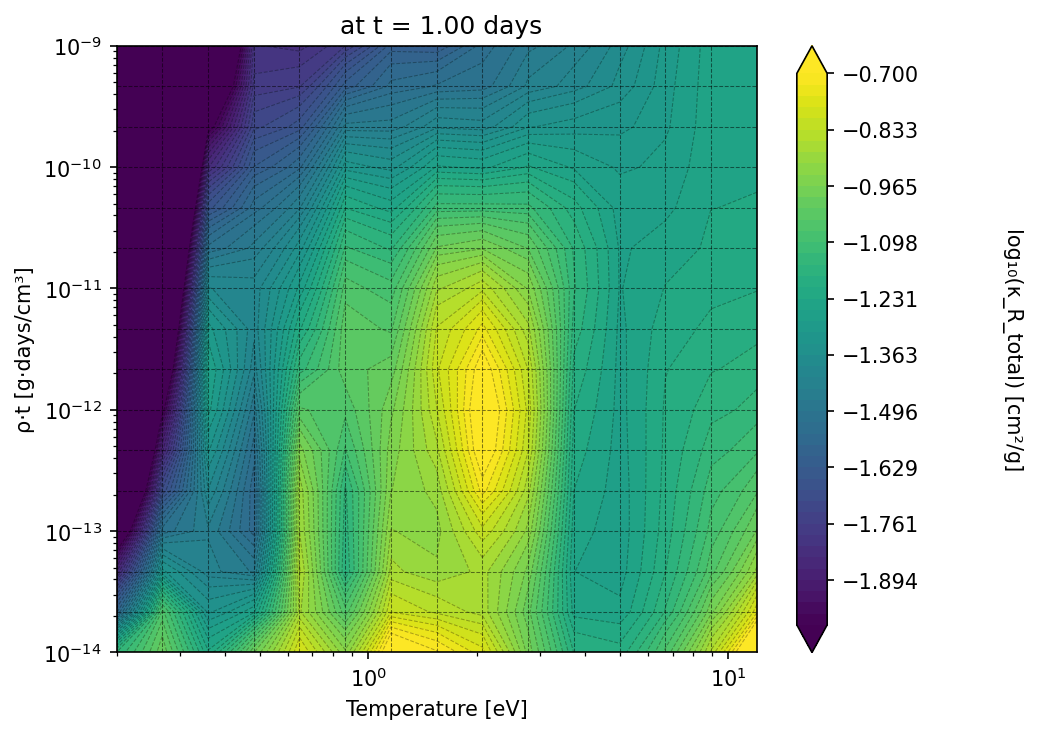
\includegraphics[width=\columnwidth]{figs/opac_map_rhot_T/t_1days.png}\\[0.35em]
    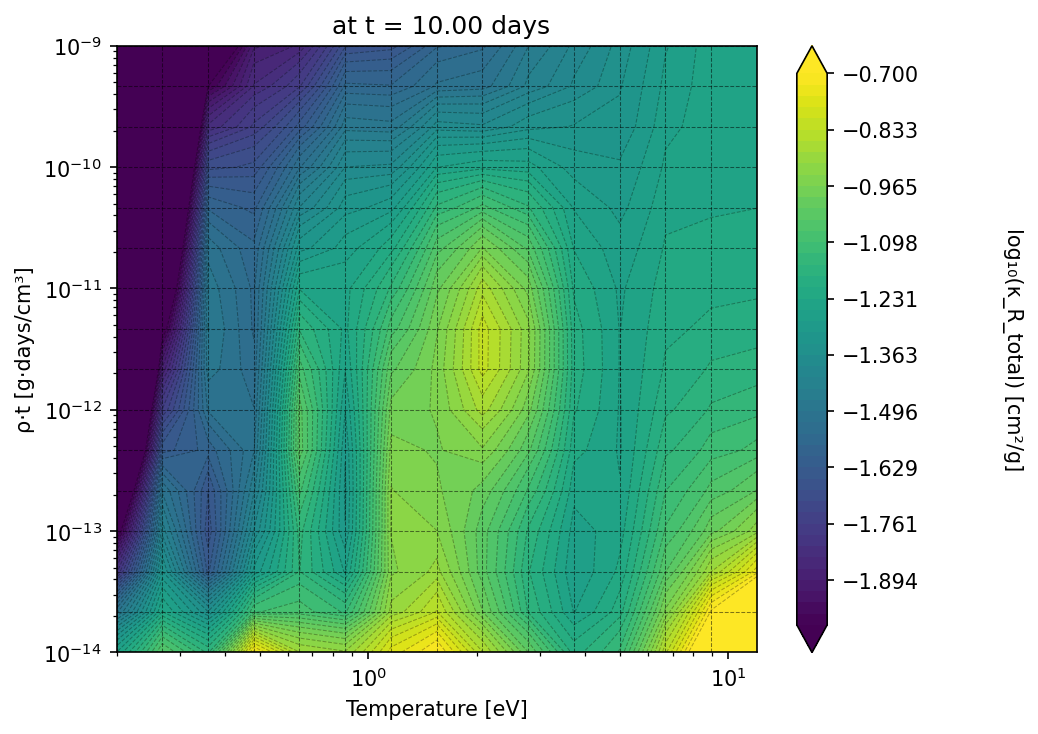
\includegraphics[width=\columnwidth]{figs/opac_map_rhot_T/t_10days.png}\\[0.35em]
    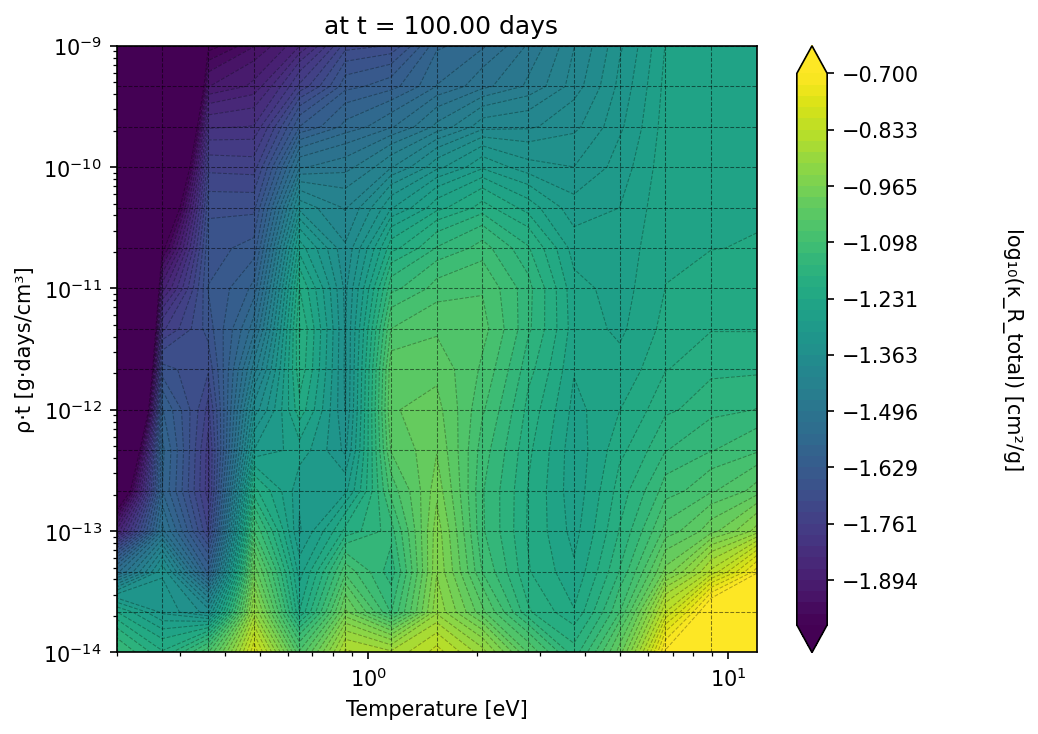
\includegraphics[width=\columnwidth]{figs/opac_map_rhot_T/t_100days.png}
    \caption{Effective expansion Rosseland mean opacity for nickel as a function of temperature and $\rho \cdot t$ at t = 1, 10, and 100 days 
    (from top to bottom). The $\rho \cdot t$ parameter is more natural for expanding media and better illustrates the scaling 
    behavior of expansion opacity.}
    \label{fig:opac_rhot_T}
    \end{figure}
    \clearpage

    \fi

    \begin{figure}[h]
        % How to create (run from python_opac_calc2):
        % cd ~/Documents/PHD/URILIGHT/python_opac_calc2
        % python plot_opac_cont.py -d opac_libs/Ni_table -t 10 -yl 1e-16 1e-11 -c 1e-3 10 --planck-rosseland --png
        % cp t_10days_rosseland.png t_10days_planck.png t_10days_ratio.png <build_paper>/figs/ as ni_rosseland_t10d.png, sn1a_planck_t10d.png, sn1a_ratio_t10d.png
        \centering
        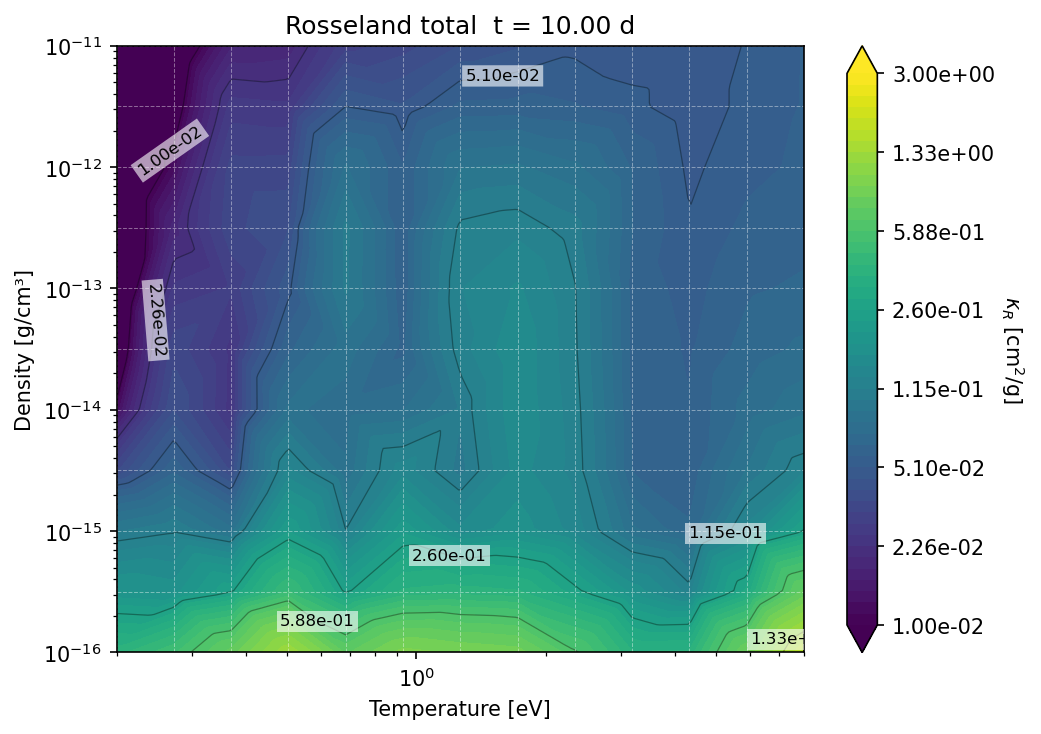
\includegraphics[width=\columnwidth]{figs/ni_rosseland_t10d.png}\\[0.35em]
        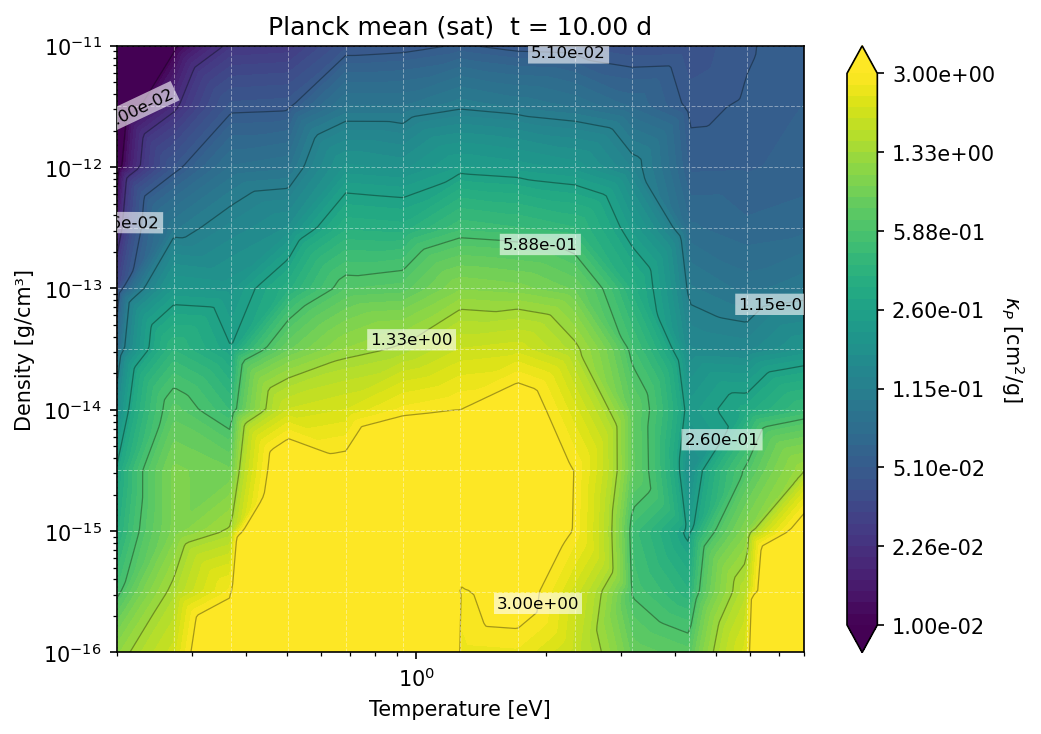
\includegraphics[width=\columnwidth]{figs/ni_planck_t10d.png}\\[0.35em]
        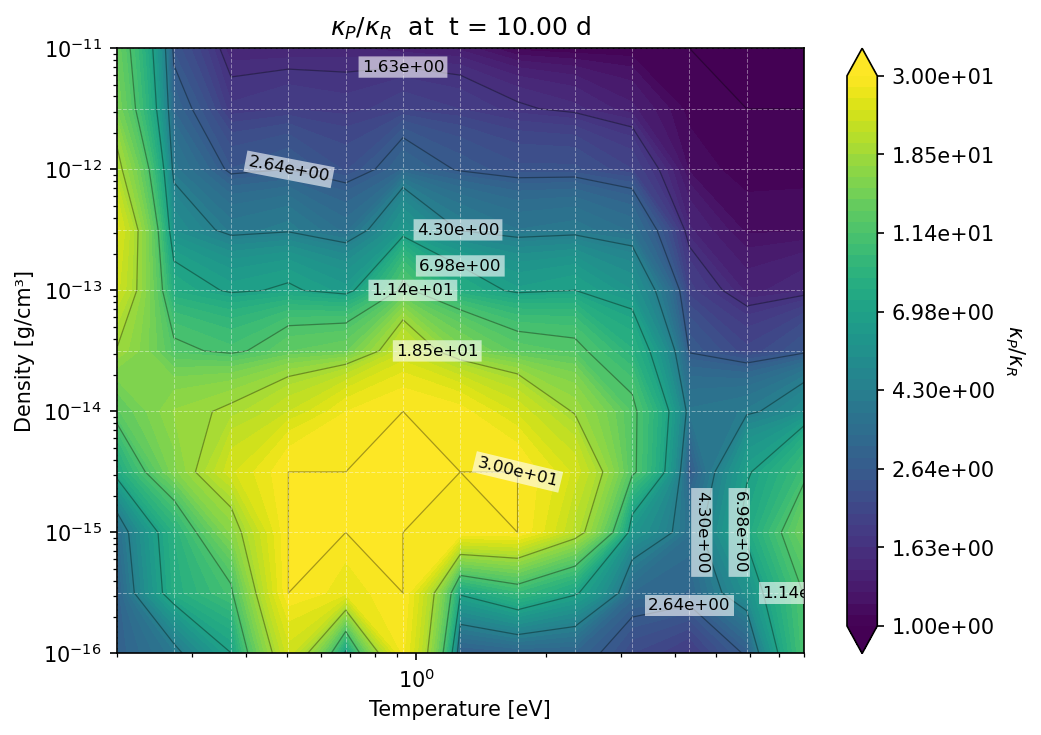
\includegraphics[width=\columnwidth]{figs/ni_ratio_t10d.png}
        \caption{Type~Ia supernova composition at $t=10$~days: Rosseland mean (top), Planck mean (middle), and $\kappa_P/\kappa_R$ ratio (bottom).
        Density $10^{-16}$--$10^{-11}$~g/cm$^3$, contour limits $\kappa \in [10^{-3}, 10]$~cm$^2$/g.}
        \label{fig:rosseland_planck_ni}
        \end{figure}


    \begin{figure}[h]
    % How to create (run from python_opac_calc2):
    % cd ~/Documents/PHD/URILIGHT/python_opac_calc2
    % python plot_opac_cont.py -d opac_libs/kilonova_table_SeTe -t 1 -yl 1e-14 1e-9 -c 1e-3 10 --planck-rosseland --png
    % cp t_1days_rosseland.png t_1days_planck.png t_1days_ratio.png <build_paper>/figs/ as kilonova_rosseland_t1d.png, kilonova_planck_t1d.png, kilonova_ratio_t1d.png
    \centering
    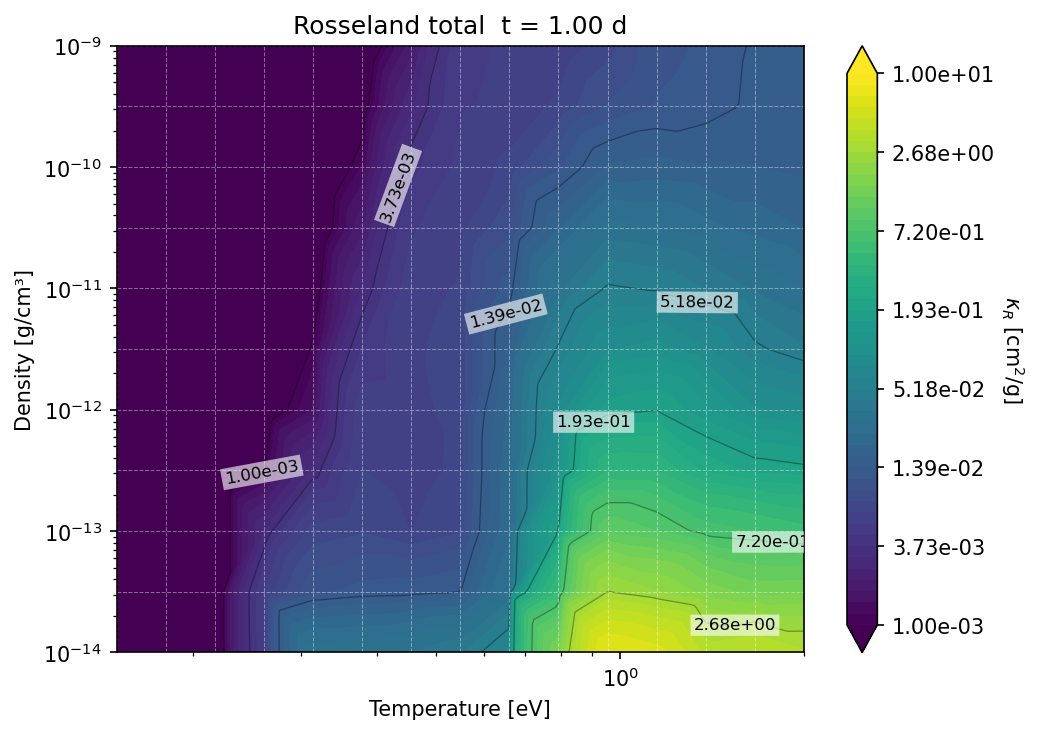
\includegraphics[width=\columnwidth]{figs/kilonova_rosseland_t1d.png}\\[0.35em]
    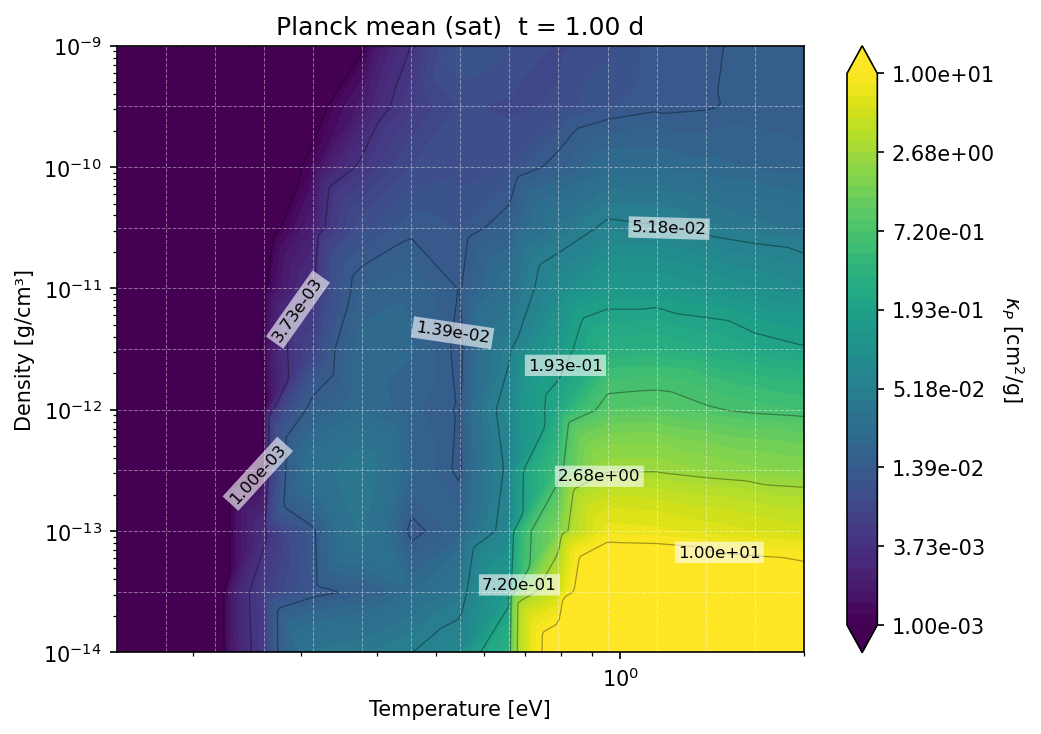
\includegraphics[width=\columnwidth]{figs/kilonova_planck_t1d.png}\\[0.35em]
    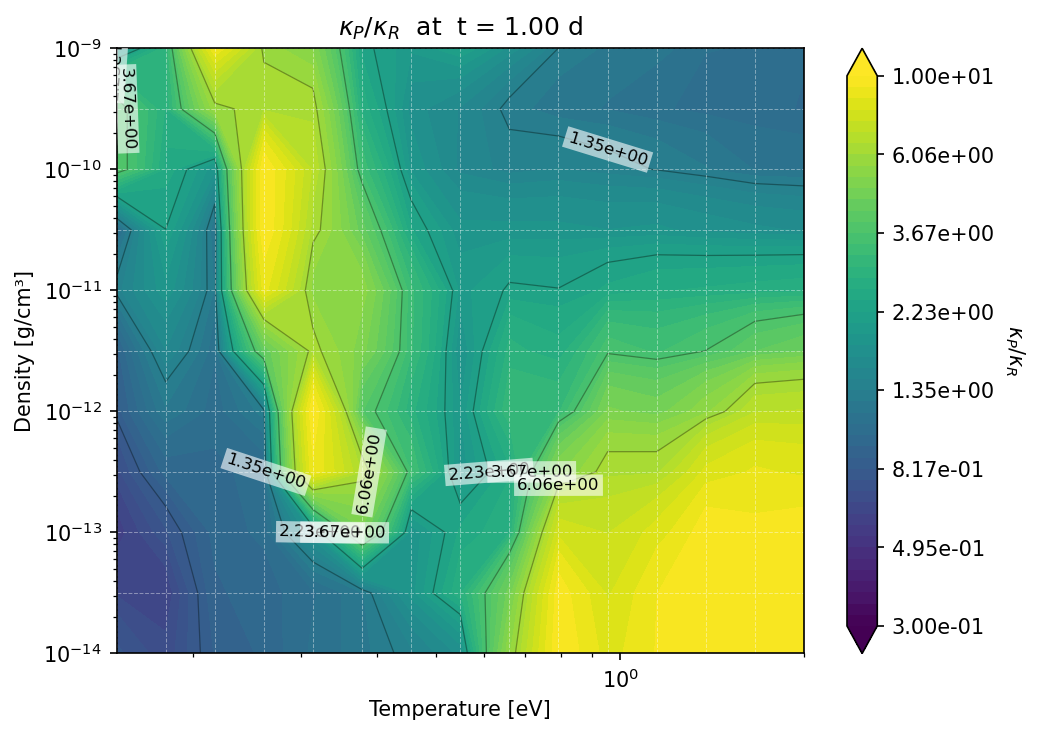
\includegraphics[width=\columnwidth]{figs/kilonova_ratio_t1d.png}
    \caption{Kilonova composition at $t=1$~day: Rosseland mean (top), Planck mean (middle), and $\kappa_P/\kappa_R$ ratio (bottom). 
    Density $10^{-14}$--$10^{-9}$~g/cm$^3$, contour limits $\kappa \in [10^{-3}, 10]$~cm$^2$/g.}
    \label{fig:rosseland_planck_kilonova}
    \end{figure}


    \clearpage




\section{Validation}
\label{SecValidation}

    Monte Carlo radiative transfer simulations using the new Rosseland mean opacity calculated from the $\tau=1$ window algorithm 
    yield results similar to full frequency-group calculations. The simulations were performed using URILIGHT \cite{urilight1,urilight2}, 
    an open-source Monte Carlo radiative transfer code designed for supernova ejecta. URILIGHT solves the time-dependent radiative 
    transfer equation in expanding media using a Monte Carlo approach, tracking photon packets through the ejecta and accounting 
    for bound-bound, free-free and thomson opacity sources.

    In \figref{fig:comparison} we compare the results of the new Rosseland mean opacity to the full frequency-group calculations. 
    We performed two types of simulations. The first uses 100 cells with an exponential decay density profile, representing 
    a more realistic supernova structure. This simulation shows reasonable but not perfect agreement (approximately 25\% deviation) 
    with the full frequency-group calculations. The discrepancy arises because as the temperature decreases from the center of the 
    supernova toward the outer regions, photons emitted in the center have a higher probability of being absorbed, since the opacity 
    to high frequencies is generally higher. This effect is not captured in the gray simulation because the gray formalism does not 
    account for temperature gradients.

    To test this hypothesis, we performed a second simulation using a single cell with a single temperature. For this case, the gray 
    model shows much better agreement with the full frequency-group calculations, confirming that the gray formalism works well when 
    temperature gradients are absent. This demonstrates that the averaging process successfully captures 
    the essential physics of expansion opacity, at least for the case of constant temperature.

    \begin{figure}[h]
    \centering
    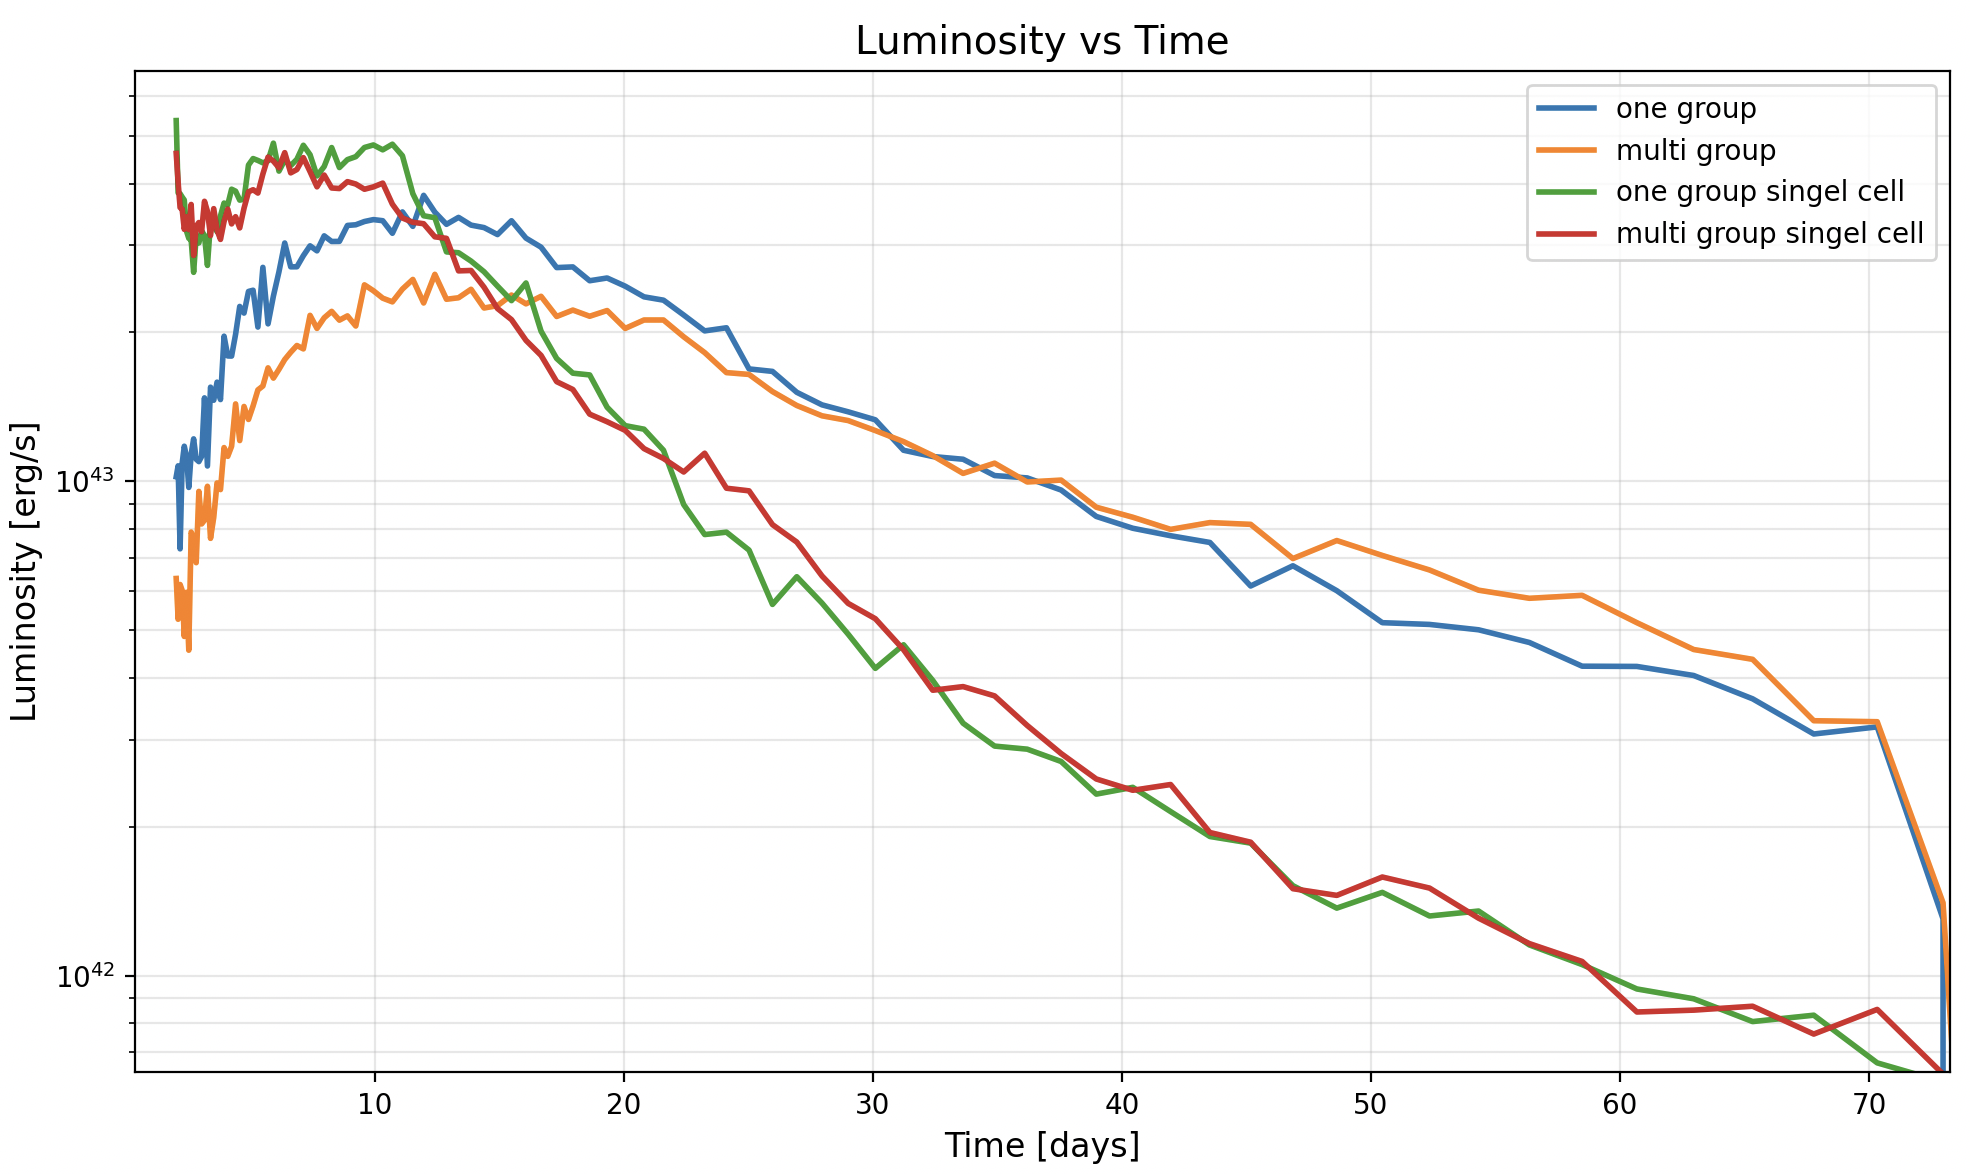
\includegraphics[width=0.48\textwidth]{figs/opacity_comparison.png}
    \caption{Comparison of Monte Carlo radiative transfer results using the new Rosseland mean opacity (from $\tau=1$ window 
    algorithm) versus full frequency-group calculations. Left: 100-cell simulation with exponential density profile showing 
    approximately 25\% deviation. Right: single-cell simulation with uniform temperature showing excellent agreement. The 
    discrepancy in the multi-cell case arises from temperature gradients, which the gray formalism does not account for.}
    \label{fig:comparison}
    \end{figure}

    % Figure was created on the cluster:
    % python plot_lum_with_deposition.py 
    % and copied here by:
    % scp roeey@10.10.10.4:/home/roeey/LIGHTBITS/SN/urilight/exp/kilonova/KN_comp1/4mats/faster/more_phot/more_time/luminosity_with_deposition.png  figs/
    \figref{fig:luminosity_kilonova} shows the same comparison as \figref{fig:comparison} for kilonova ejecta: Monte Carlo radiative transfer with the new Rosseland mean opacity versus full frequency-group calculations.

    \begin{figure}[h]
    \centering
    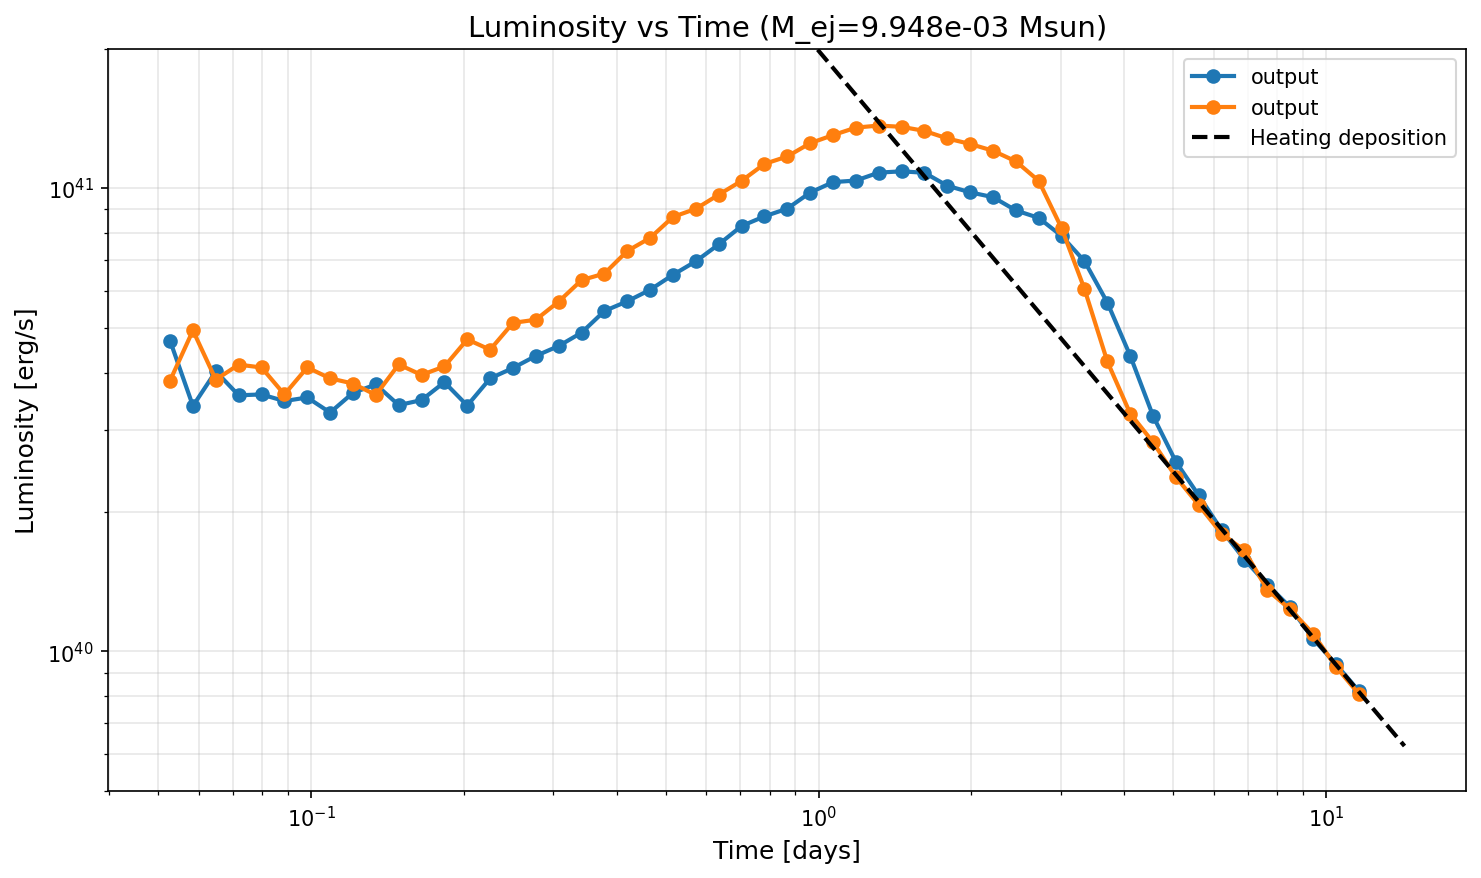
\includegraphics[width=0.48\textwidth]{figs/luminosity_with_deposition.png}
    \caption{Same layout as \figref{fig:comparison} for kilonova ejecta: comparison of luminosity (with energy deposition) from Monte Carlo simulations using the new Rosseland mean opacity versus full frequency-group calculations.}
    \label{fig:luminosity_kilonova}
    \end{figure}

\section{Summary}
\label{SecSummary}

We have presented a new algorithm for calculating Rosseland mean opacity that accounts for expansion opacity effects from 
bound-bound atomic transitions. The method uses a $\tau=1$ window to smooth the frequency-dependent opacity, with the smoothed 
value calculated as $\kappa = 1/(\rho \Delta x)$ where $\Delta x$ is the path length to reach optical depth unity. Validation 
through Monte Carlo simulations confirms that this approach captures the essential physics while enabling efficient gray 
opacity calculations.

The Python code for building opacity tables using this algorithm is available at 
\url{https://github.com/roee2000/expansion_opacity_calculation}.

\bibliographystyle{elsarticle-num}
\bibliography{refs}

\end{document}
